% 5-panel Overall Architecture (draft). Needs tikz, graphicx and paper/figures/pgct_style.tex.
% Images: make_assets.py (real renderer crops; real discovery log). Bars and value curves are illustrations.
\begin{tikzpicture}[pg,every node/.append style={execute at begin node={\hyphenpenalty10000\relax}}]
\tikzset{
  panel/.style={draw=pgblue,line width=.8pt,rounded corners=3pt,fill=white,minimum height=6.0cm,anchor=north},
  head/.style={fill=pgblue,text=white,font=\sffamily\small\bfseries,align=center,rounded corners=3pt,
               minimum height=.95cm,anchor=north,inner sep=2pt},
  note/.style={font=\sffamily\scriptsize,align=center,text=black},
  capt/.style={font=\sffamily\tiny,text=pggrey,align=center},
}
\def\W{3.05}
% x centres of the panels
\def\xa{0}\def\xb{3.55}\def\xc{7.1}\def\xd{10.65}\def\xe{15.05}
% ---------- panel frames and headers
\foreach \x/\w/\t [count=\n] in {\xa/\W/{Independent\\Learning},\xb/\W/{Independent\\Reward Modeling},
                                  \xc/\W/{Common\\Reward Probing},\xd/\W/{Latent Team\\Identification},
                                  \xe/4.75/{Selective Critic\\Utilization \& Max-GAE}} {
  \node[panel,minimum width=\w cm] (p\n) at (\x,0) {};
  \node[head,text width=\w cm-4pt] (h\n) at (\x,0) {\t};
  \node[num,fill=white,text=pgblue] at (h\n.north west) {\n};
}
\foreach \a/\b in {p1/p2,p2/p3,p3/p4,p4/p5} {\draw[flow] (\a.east) -- (\b.west);}
% ---------- 1. independent learning: real renderer crop
\node[inner sep=0] (img1) at (\xa,-2.3) {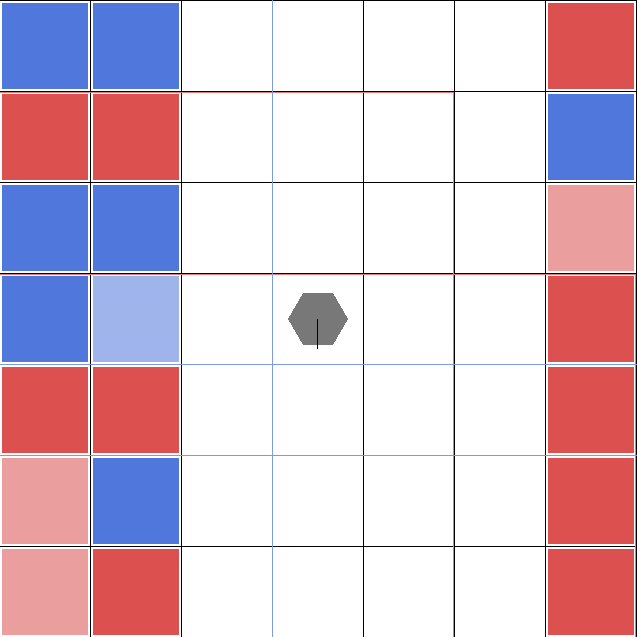
\includegraphics[width=2.3cm]{agent_scene.png}};
\node[capt,below=1pt of img1] {RWARE, agent $i$ (grey);\\shelf colours: true teams, hidden};
\node[note,text width=2.8cm] at (\xa,-4.95) {own observation $o_{i,t}$,\\own action, own reward $r_i$\\[2pt]PPO Actor \& Critic};
% ---------- 2. reward modeling: public views before/after (real renderer, private colours removed)
\node[inner sep=0] (u0) at (\xb-0.72,-1.75) {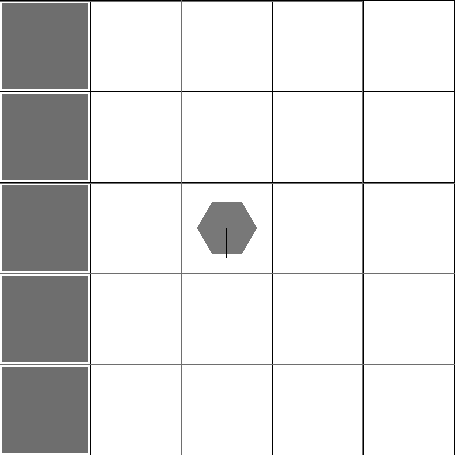
\includegraphics[width=1.2cm]{agent_view_t0.png}};
\node[inner sep=0] (u1) at (\xb+0.72,-1.75) {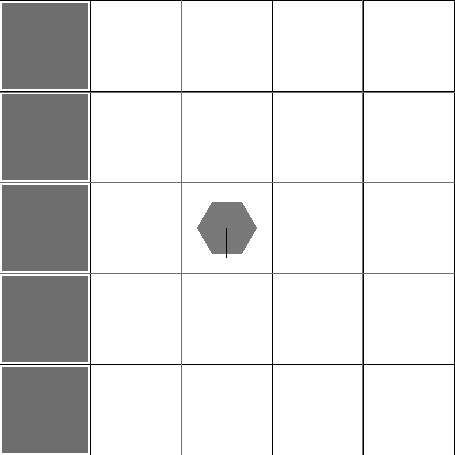
\includegraphics[width=1.2cm]{agent_view_t1.png}};
\draw[flowg] (u0) -- node[lbl,above=-1pt]{$a_t$} (u1);
\node[capt,below=0pt of u0] {$u_t$};\node[capt,below=0pt of u1] {$u_{t+1}$};
\node[box,minimum width=1.6cm,inner sep=2pt,font=\sffamily\scriptsize] (mlp) at (\xb,-3.35) {MLP $\widehat r_i$};
\draw[flowg] ($(u0.south)+(0,-.25)$) -- (mlp); \draw[flowg] ($(u1.south)+(0,-.25)$) -- (mlp);
\node[note] (rhat) at (\xb,-4.05) {$\widehat r_i(u_t,a_t,u_{t+1}) \approx r_i$};
\draw[flowg] (mlp) -- (rhat);
\node[note,text width=2.8cm] at (\xb,-5.0) {public view only\\(no team, request,\\or reward exchanged)};
% ---------- 3. common reward probing: both agents' events + mirror, two predictors answer
\node[card,fill=pgsky,text width=1.15cm,font=\sffamily\tiny] (ei) at (\xc-0.72,-1.4) {events\\of $i$};
\node[card,fill=pgsand,text width=1.15cm,font=\sffamily\tiny] (ej) at (\xc+0.72,-1.4) {events\\of $j$};
\node[card,fill=pglight,text width=2.6cm,font=\sffamily\tiny] (mm) at (\xc,-2.05) {+ left--right mirrors $\to$ probes $\mathcal Q_{ij}$};
\begin{scope}[shift={(\xc-1.25,-3.95)}]
  \draw[pggrey,line width=.4pt] (0,0) -- (2.5,0);
  \foreach \h/\c [count=\k] in {1/pgblue,0.08/pgorange,0.05/pgblue,0.95/pgorange} {
    \fill[\c] ({0.35+0.5*(\k-1)+(\k>2?0.25:0)},0) rectangle ++(0.32,{1.15*\h});}
  \node[capt,anchor=north] at (0.75,-0.02) {event};
  \node[capt,anchor=north] at (1.95,-0.02) {mirror};
\end{scope}
\node[capt] at (\xc,-2.55) {\textcolor{pgblue}{$\widehat r_i$} vs \textcolor{pgorange}{$\widehat r_j$} on the same probes};
\node[note,text width=2.8cm] at (\xc,-4.75) {different responses\\$\Rightarrow$ distance $D_{ij}\approx1$\\(teammates: $D_{ij}\approx0$)};
\node[capt] at (\xc,-5.65) {bars: illustration};
% ---------- 4. latent team identification: real log
\node[inner sep=0] (ema) at (\xd,-2.6) {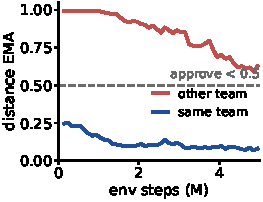
\includegraphics[width=2.9cm]{discovery_ema.pdf}};
\node[note,text width=2.8cm] at (\xd,-4.65) {approve if EMA $<0.5$,\\both mature, $\ge3$ rounds;\\otherwise abstain};
\node[capt] at (\xd,-5.65) {real log: seed 1, 5M steps};
% ---------- 5. selective critic & Max-GAE
\begin{scope}[shift={(\xe-2.05,-1.95)}]
  \node[circle,draw=pgblue,fill=white,font=\sffamily\scriptsize,inner sep=1pt,minimum size=5mm] (ri) at (0.45,0) {$i$};
  \node[circle,draw=pgblue,fill=pgsky,font=\sffamily\scriptsize,inner sep=1pt,minimum size=5mm] (rj) at (1.55,0.45) {$j$};
  \node[circle,draw=pggrey,fill=white,font=\sffamily\scriptsize,inner sep=1pt,minimum size=5mm] (rk) at (1.55,-0.45) {$k$};
  \draw[flow,pggreen,draw=pggreen] (rj) -- (ri);
  \draw[pggrey,dashed,line width=.7pt] (rk) -- (ri);
  \node[capt,anchor=west,align=left] at (1.9,0.45) {approved\\\& met: donor};
  \node[capt,anchor=west,align=left] at (1.9,-0.45) {not approved};
\end{scope}
\begin{scope}[shift={(\xe-2.05,-4.05)}]
  \draw[pggrey,line width=.4pt,->] (0,0) -- (2.35,0) node[capt,anchor=north east] {my history $t$};
  \fill[pgsand] plot[smooth] coordinates {(0.1,0.35) (0.7,0.55) (1.3,0.5) (2.2,0.85)}
       -- plot[smooth] coordinates {(2.2,1.3) (1.3,1.25) (0.7,1.05) (0.1,0.75)} -- cycle;
  \draw[pgblue,line width=1pt] plot[smooth] coordinates {(0.1,0.35) (0.7,0.55) (1.3,0.5) (2.2,0.85)};
  \draw[pgorange,line width=1pt] plot[smooth] coordinates {(0.1,0.75) (0.7,1.05) (1.3,1.25) (2.2,1.3)};
  \node[capt,text=pgorange,anchor=south west] at (0.0,1.35) {$\max_j V_j(\tilde h_{i,t})$};
  \node[capt,text=pgblue,anchor=north west] at (1.25,0.45) {$V_i(h_{i,t})$};
  \node[font=\sffamily\scriptsize\bfseries,text=pgorange] at (1.0,0.82) {$b$};
\end{scope}
\node[box,text width=1.6cm,font=\sffamily\scriptsize,inner sep=2pt] (act) at (\xe+1.45,-3.25) {\textbf{Actor}\\$A^{\rm PGCT}$\\(Max-GAE)};
\node[box,text width=1.6cm,font=\sffamily\scriptsize,inner sep=2pt] (cri) at (\xe+1.45,-4.75) {\textbf{Critic}\\own return};
\draw[flowo] ($(\xe+0.35,-3.25)$) -- (act);
\node[capt,text width=4.4cm] at (\xe,-5.65) {no approved teammate met $\Rightarrow$ update equals IPPO\\curves: illustration};
% ---------- Q1 / Q2 bands
\begin{scope}[on background layer]
\node[band,fill=pgsky,fit=(p1)(p4),inner sep=5pt,label={[font=\sffamily\small\bfseries,text=pgblue,anchor=south west]north west:Q1. Discover latent teammates from own reward}] {};
\node[band,fill=pgsand,fit=(p5),inner sep=5pt,label={[font=\sffamily\small\bfseries,text=pgorange,anchor=south east]north east:Q2. Use them in learning}] {};
\end{scope}
% ---------- contact strip and loop
\node[note,anchor=north,text width=19cm,align=center] at (7.5,-6.55) {%
  \textbf{On contact} \quad \textcolor{pggreen}{\textbf{sent:}} public event views, predictions, Critic weights
  \qquad \textcolor{pgorange}{\textbf{not sent:}} reward values, team labels, Actor weights
  \qquad \textcolor{pggrey}{(repeated every rollout)}};
\end{tikzpicture}
